\documentclass{article}
\usepackage[landscape]{geometry}
\usepackage{url}
\usepackage{multicol}
\usepackage{amsmath}
\usepackage{esint}
\usepackage{amsfonts}
\usepackage{tikz}
\usetikzlibrary{decorations.pathmorphing}
\usepackage{amsmath,amssymb}

\usepackage{colortbl}
\usepackage{xcolor}
\usepackage{mathtools}
\usepackage{amsmath,amssymb}
\usepackage{enumitem}
\makeatletter

\newcommand*\bigcdot{\mathpalette\bigcdot@{.5}}
\newcommand*\bigcdot@[2]{\mathbin{\vcenter{\hbox{\scalebox{#2}{$\m@th#1\bullet$}}}}}
\makeatother

\title{Signal Analysis Formulae Sheet}
\usepackage[english]{babel}
\usepackage[utf8]{inputenc}

\advance\topmargin-.8in
\advance\textheight3in
\advance\textwidth3in
\advance\oddsidemargin-1.45in
\advance\evensidemargin-1.45in
\parindent0pt
\parskip2pt
\newcommand{\hr}{\centerline{\rule{3.5in}{1pt}}}
% \colorbox[HTML]{e4e4e4}{\makebox[\textwidth-2\fboxsep][l]{texto}}
\begin{document}

\begin{center}{\huge{\textbf{Signal Analysis Formula Sheet}}}\\
\end{center}
\begin{multicols*}{2}

\tikzstyle{mybox} = [draw=black, fill=white, very thick,
    rectangle, rounded corners, inner sep=10pt, inner ysep=10pt]
\tikzstyle{fancytitle} =[fill=black, text=white, font=\bfseries]


%%%%%%%%%%%%%%%%%%%%%%%%%%%%%%%%%%%%%%%%%%%%%%%%%%%%%%%%%%%%%%%%%%%%%%%%%%%%%%%%%%%%%%%%%%%%%%%%%%%%%%%%%%%%%%%%%%
%  Continuous Time
%%%%%%%%%%%%%%%%%%%%%%%%%%%%%%%%%%%%%%%%%%%%%%%%%%%%%%%%%%%%%%%%%%%%%%%%%%%%%%%%%%%%%%%%%%%%%%%%%%%%%%%%%%%%%%%%%%

%%%%%%%%%%%%%%%%%%%%%%%%%%%%%%%%%%%%%%%%%%%%%%%%%%%%%%%%%%%%%%%%%%%%%%%%%%%%%%%%%%%%%%%%%%%%%%%%%%%%%%%%%%%%%%%%%%
%------------ Continuous Time - Chapter 2-3 ---------------
\begin{tikzpicture}
\node [mybox] (box){%
    \begin{minipage}{0.46\textwidth}
    
	\begin{tabular}{lp{8cm} l}
        Trasformata di Fourier:
        $ X(f) = \int_{-\infty}^{\infty} x(t) \cdot e^{-j2\pi ft} \, dt $ \\
        Periodic signal: 
        $x(t) = \sum_{n=-\infty}^{\infty} x(t + nT)$\\
        Inner product:
        $\langle \mathbf{v}, \mathbf{w} \rangle = \sum_{i=1}^n v_i w_i$\\
        Parseval's Rule:
        $ \int_{-\infty}^{\infty} |x(t)|^2 \, dt = \int_{-\infty}^{\infty} |X(f)|^2 \, df $ \\
        Spettro di potenza:
        $S_x(f) = |X(f)|^2$\\
        Valore Medio:
        $\bar{x} = \lim_{{T \to \infty}} \frac{1}{T} \int_{-T/2}^{T/2} x(t) \, dt$\\
        Energy of a signal:
        $E = \int_{-\infty}^{\infty} |x(t)|^2 \, dt$\\
        Power of a periodic signal:
        $ P = \lim_{{T \to \infty}} \frac{1}{T} \int_{-T/2}^{T/2} |x(t)|^2 \, dt $ \\
        Time Average:
        $\bar{x} = \frac{1}{T2 - T1} \int_{T1}^{T2} x(t) \, dt$\\
        Instantaneous Power:
        $P(t_0) = |x(t_0)|^2$\\
        Scalar Product:
        $\langle x, y \rangle = \int x(t) \cdot y(t) \, dt$\\
        Norm:
        $\|x\| = \sqrt{\int |x(t)|^2 \, dt}$\\
        Orthogonality:
        $\langle x, y \rangle = 0$\\
	\end{tabular}
	
    \end{minipage}
};
%------------ Continuous Time - Chapter 2-3 HEADER ---------------
\node[fancytitle, right=10pt] at (box.north west) {Countinuous Time - Chapter 2-3};
\end{tikzpicture}



%%%%%%%%%%%%%%%%%%%%%%%%%%%%%%%%%%%%%%%%%%%%%%%%%%%%%%%%%%%%%%%%%%%%%%%%%%%%%%%%%%%%%%%%%%%%%%%%%%%%%%%%%%%%%%%%%%
%------------ Continuous Time - Chapter 4 ---------------
\begin{tikzpicture}
\node [mybox] (box){%
    \begin{minipage}{0.46\textwidth}
    
	\begin{tabular}{lp{8cm} l}
        Schwarz's Inequality (Cauchy-Schwarz Inequality):\\
        For vectors u and v in an inner product space, it states:\\
        $|\langle u, v \rangle|^2 \leq \langle u, u \rangle \cdot \langle v, v \rangle$\\

        Orthonormal Set:\\
        An orthonormal set ${u_i}$ is a set of vectors in an inner product space such that:\\
        $\langle u_i, u_j \rangle = \delta_{ij}$\\

        Orthonormal Basis:\\
        An orthonormal basis is a set of vectors that is both orthonormal and forms a\\
        basis for the vector space. If ${u_i}$ is an orthonormal basis, then for any \\
        vector v in the space:\\
        $v = \sum_{i} \langle v, u_i \rangle \cdot u_i$\\

        Gram-Schmidt: \\

        Canonical bases:\\
        $x(t) \approx x_0(t) = \sum_{n=-\infty}^{\infty} x(n\Delta t) \Pi_{\Delta t}(t - n\Delta t)$ \\


	\end{tabular}
	
    \end{minipage}
};
%------------ Continuous Time - Chapter 4 HEADER ---------------
\node[fancytitle, right=10pt] at (box.north west) {Countinuous Time - Chapter 4};
\end{tikzpicture}



%%%%%%%%%%%%%%%%%%%%%%%%%%%%%%%%%%%%%%%%%%%%%%%%%%%%%%%%%%%%%%%%%%%%%%%%%%%%%%%%%%%%%%%%%%%%%%%%%%%%%%%%%%%%%%%%%%
%------------ Continuous Time - Chapter 5 ---------------
\begin{tikzpicture}
\node [mybox] (box){%
    \begin{minipage}{0.46\textwidth}
    
	\begin{tabular}{lp{8cm} l}
        Fourier Basis:  
        $e^{j\omega t}$\\

        Where:\\
        - $e$ is the base of the natural logarithm (approximately 2.71828).\\
        - $j$ represents the imaginary unit ($j^2 = -1$).\\
        - $\omega$ is the angular frequency (measured in radians per second).\\
        - $t$ is time.\\


	\end{tabular}
	
    \end{minipage}
};
%------------ Continuous Time - Chapter 5 HEADER ---------------
\node[fancytitle, right=10pt] at (box.north west) {Countinuous Time - Chapter 5};
\end{tikzpicture}

\newcolumn



%%%%%%%%%%%%%%%%%%%%%%%%%%%%%%%%%%%%%%%%%%%%%%%%%%%%%%%%%%%%%%%%%%%%%%%%%%%%%%%%%%%%%%%%%%%%%%%%%%%%%%%%%%%%%%%%%%
%  Discrete Time
%%%%%%%%%%%%%%%%%%%%%%%%%%%%%%%%%%%%%%%%%%%%%%%%%%%%%%%%%%%%%%%%%%%%%%%%%%%%%%%%%%%%%%%%%%%%%%%%%%%%%%%%%%%%%%%%%%


%%%%%%%%%%%%%%%%%%%%%%%%%%%%%%%%%%%%%%%%%%%%%%%%%%%%%%%%%%%%%%%%%%%%%%%%%%%%%%%%%%%%%%%%%%%%%%%%%%%%%%%%%%%%%%%%%%
%------------ Discrete Time - Chapter 1 ---------------
\begin{tikzpicture}
\node [mybox] (box){%
    \begin{minipage}{0.46\textwidth}
    
	\begin{tabular}{lp{8cm} l}
        Trasformata di Fourier Discreta (DFT):
        $X[k] = \sum_{n=0}^{N-1} x[n] \cdot e^{-j2\pi kn/N}$ \\
        Parseval's Rule Discrete Time:
        $ \sum_{n=0}^{N-1} |x[n]|^2 = \frac{1}{N} \sum_{k=0}^{N-1} |X[k]|^2 $\\

        Base di Fourier per sequenze periodiche:\\
        La base di Fourier per sequenze periodiche è utilizzata per rappresentare \\
        segnali discreti periodici di lunghezza N. I componenti della base includono \\
        armoniche discrete:

   
        $e_k[n] = e^{j\frac{2\pi kn}{N}}, \quad k = 0, 1, 2, \ldots, N-1$\\
   

        Dove:\\
        - $e$ è la base dell'esponenziale complesso.\\
        - $j$ rappresenta l'unità immaginaria.\\
        - $k$ è un intero che rappresenta l'armonica.\\
        - $n$ è l'indice temporale discreto.\\

        Gram-Schmidt:\\

        1. Ortogonalizzazione:    
        $u_i = v_i - \sum_{j=1}^{i-1} \frac{\langle v_i, u_j \rangle}{\langle u_j, u_j \rangle}u_j$\\
   

        2. Normalizzazione (Ortonormalizzazione):
        $u_i = \frac{u_i}{\|u_i\|}$\\
        
        \end{tabular}
	
    \end{minipage}
};
%------------ Discrete Time - Chapter 1 HEADER ---------------
\node[fancytitle, right=10pt] at (box.north west) {Discrete Time - Chapter 1};
\end{tikzpicture}



%%%%%%%%%%%%%%%%%%%%%%%%%%%%%%%%%%%%%%%%%%%%%%%%%%%%%%%%%%%%%%%%%%%%%%%%%%%%%%%%%%%%%%%%%%%%%%%%%%%%%%%%%%%%%%%%%%
%------------ Descrete Time - Chapter 2 ---------------
\begin{tikzpicture}
\node [mybox] (box){%
    \begin{minipage}{0.46\textwidth}
    
	\begin{tabular}{lp{8cm} l}
        Linear:  
        $y[n] = a_1y_1[n] + a_2y_2[n]$\\
        Time-invariant:  
        $y[n] = x[n] * h[n]$\\
	\end{tabular}
	
    \end{minipage}
};
%------------ Discrete Time - Chapter 2 HEADER ---------------
\node[fancytitle, right=10pt] at (box.north west) {Discrete Time - Chapter 2};
\end{tikzpicture}


%%%%%%%%%%%%%%%%%%%%%%%%%%%%%%%%%%%%%%%%%%%%%%%%%%%%%%%%%%%%%%%%%%%%%%%%%%%%%%%%%%%%%%%%%%%%%%%%%%%%%%%%%%%%%%%%%%
%  Trigonometry
%%%%%%%%%%%%%%%%%%%%%%%%%%%%%%%%%%%%%%%%%%%%%%%%%%%%%%%%%%%%%%%%%%%%%%%%%%%%%%%%%%%%%%%%%%%%%%%%%%%%%%%%%%%%%%%%%%


%%%%%%%%%%%%%%%%%%%%%%%%%%%%%%%%%%%%%%%%%%%%%%%%%%%%%%%%%%%%%%%%%%%%%%%%%%%%%%%%%%%%%%%%%%%%%%%%%%%%%%%%%%%%%%%%%%
%------------ Trigonometry ---------------
\begin{tikzpicture}
\node [mybox] (box){%
    \begin{minipage}{0.46\textwidth}
    
	\begin{tabular}{lp{8cm} l}

        Identità Trigonometriche Fondamentali:\\
        $\sin^2(\theta) + \cos^2(\theta) = 1$\\
        $\tan(\theta) = \frac{{\sin(\theta)}}{{\cos(\theta)}}$\\
        $\sec(\theta) = \frac{1}{{\cos(\theta)}}$\\
        $\csc(\theta) = \frac{1}{{\sin(\theta)}}$\\
        $\cot(\theta) = \frac{1}{{\tan(\theta)}}$\\
        Seno e Coseno di Somma e Differenza:\\
        $\sin(A + B) = \sin(A)\cos(B) + \cos(A)\sin(B)$\\
        $\cos(A + B) = \cos(A)\cos(B) - \sin(A)\sin(B)$\\
        $\sin(A - B) = \sin(A)\cos(B) - \cos(A)\sin(B)$\\
        $\cos(A - B) = \cos(A)\cos(B) + \sin(A)\sin(B)$\\
        Seno e Coseno dell'Angolo Duplo:
        $\sin(2\theta) = 2\sin(\theta)\cos(\theta)$\\
        $\cos(2\theta) = \cos^2(\theta) - \sin^2(\theta) = 2\cos^2(\theta) - 1 = 1 - 2\sin^2(\theta)$\\
        Seno e Coseno dell'Angolo Metà:
        $\sin\left(\frac{\theta}{2}\right) = \pm \sqrt{\frac{1 - \cos(\theta)}{2}}$\\
        $\cos\left(\frac{\theta}{2}\right) = \pm \sqrt{\frac{1 + \cos(\theta)}{2}}$\\
        Formule delle Funzioni Inverse:
        $\sin^{-1}(x) + \cos^{-1}(x) = \frac{\pi}{2}$\\
        $\tan^{-1}(x) + \cot^{-1}(x) = \frac{\pi}{2}$\\
        Formule del Prodotto:
        $\sin(A)\sin(B) = \frac{1}{2}[\cos(A - B) - \cos(A + B)]$\\
        $\cos(A)\cos(B) = \frac{1}{2}[\cos(A - B) + \cos(A + B)]$\\
        Sinc:
        $\text{sinc}(x) = \frac{\sin(\pi x)}{\pi x}, \quad \text{per } x \neq 0$\\
	\end{tabular}
	
    \end{minipage}
};
%------------ Trigonometry - HEADER ---------------
\node[fancytitle, right=10pt] at (box.north west) {Trigonometry};
\end{tikzpicture}

%%%%%%%%%%%%%%%%%%%%%%%%%%%%%%%%%%%%%%%%%%%%%%%%%%%%%%%%%%%%%%%%%%%%%%%%%%%%%%%%%%%%%%%%%%%%%%%%%%%%%%%%%%%%%%%%%%

\newpage
\begin{figure}
    \centering
    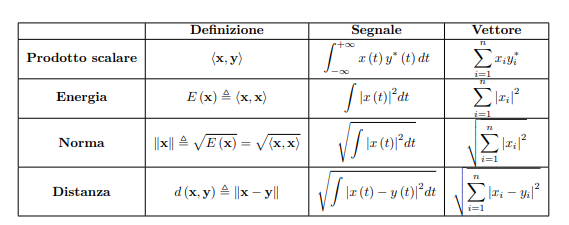
\includegraphics[width=0.15\textwidth]{./Screenshot 2023-11-07 234200.png}
\end{figure}

\end{multicols*}
\end{document}